
\subsection{Client}
Het voornaamste onderdeel van de client is het canvas-element waarin de output getekend wordt door Kinetic.js. Daarboven zit de Canvas.hs javascriptcode die de verbinding onderhoudt met de module en dit doorspeelt naar Kinetic.js om te tekenen. In dit deel worden voornamelijk de ontwerpbeslissingen besproken die betrekking hebben op de werking met KineticJS en de webbrowser.

\begin{figure}
\begin{center}
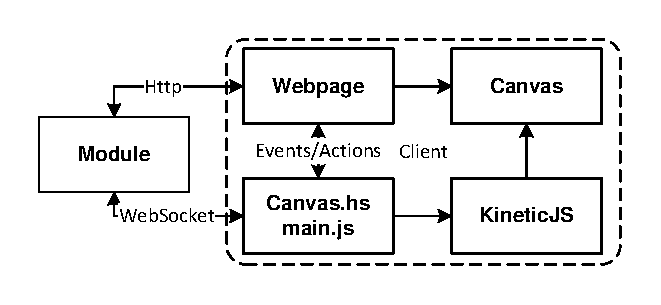
\includegraphics[keepaspectratio,width=\textwidth]{./images/client_architecture.pdf}
\caption{Architectuur van de JavaScript client}
\label{fig:architecture_client}
\end{center}
\end{figure}

\subsubsection{Canvas/Events}
Vanuit de module ontvangt de client via de WebSocket verbinding output. Ieder element wordt omgezet en aangemaakt in KineticJS. Voor elk element dat geinteresseerd is in een event wordt een eventlisteners toegevoegd. Wanneer de volledige structuur opgebouwd is wordt de oude structuur weggegooid en de nieuwe structuur op het canvas getekend.

\paragraph{Mousedrag}
Standaard ondersteunt KineticJS mousedrag events, maar door de manier waarop Canvas.hs iedere keer opnieuw de output genereert raken de events van KineticJS verloren. Daarom maakt Canvas.hs gebruik van een eigen implementatie van mousedrag in de Canvas. Een mousedrag begint met een MouseDownEvent. Vanaf dat moment houdt de client een ID bij van het huidige element. Alle opvolgende MouseMoveEvents zijn drag events die naar de client worden verstuurd. Deze MouseMoveEvents worden dooregegeven naar de Haskell kant met de vorige coördinaten van de muis en de huidige coördinaten van de muis.
Op deze manier kan de Haskell kant bepalen wat er moet gebeuren tijdens het draggen. Op het moment dat het programma aangeeft niet meer geinteresseerd te zijn in drag events op dat ID of in het geval van een MouseUpEvent stopt de drag in de client.

\subsubsection{Acties}
De programmeur kan een aantal specifieke acties uitvoeren op de client. De state van deze acties wordt onderhouden door de client zelf.
\todo{Referentie naar de specifieke sectie in de grafische bibliotheek}

\paragraph{Browserrestricties}
Canvas.hs biedt de optie om de canvas in volledigscherm te laten weergeven. Door veiligheidsfunctionaliteiten in de huidige webbrowsers is het niet mogelijk om direct naar volledigscherm te gaan met behulp van JavaScript. Dit is alleen mogelijk vanuit klik- en toetsenbordevents. Daarom krijgt de gebruiker eerst een menu te zien voordat de browser naar volledigscherm gaat. Dezelfde veiligheidsrestricties zijn er voor het bestandenselectiemenu, hierdoor heeft Canvas.hs daar ook een menu voor.

\todo{Referentie naar de grafische bibliotheek over volledigscherm}

\paragraph{Debug Console}
Voor de programmeur die gebruik gaat maken van de Canvas.hs library is het belangrijk dat zijn interface er zo uit ziet zoals hij dit wil. Ongetwijfeld zal een programmeur tegen problemen aanlopen bij het bouwen van de interface die hij niet had voorzien bij het schrijven van zijn code. Om probleemoplossing hiervan te vergemakkelijken bevat Canvas.hs een debug console bevat waar het aanroepen van teken functies en de invloed van deze API aanroepen goed visueel en tekstueel inzichtelijk worden. Doormiddel van een actie vanuit het programma van de gebruiker kan de debug console tevoorschijn gehaald worden.